\section{Approach}
\label{sec:approach}

%\begin{itemize}
%\item how to extract the word pairs encoded causal
%relations from web corpus
%
%\item propose how to compute causality
%strength between words
%   i) word association strength
%   ii) introduce cause / effect role using
%	extracted data set
%   iii) propose a novel causality strength
%	metric between words
%
%\item combination approach to apply to compute
%causality strength between short texts
%\item treat short text as bag of words, all pairs, sum up, normalize
%\end{itemize}

To reason about causality between short texts,
our framework includes i) a network of causal relation weighted with
causality co-occurrences between terms that is extracted from
a large web corpus; ii) a novel metric to compute causality strength
 between any two terms based on this network; iii)
a simple algorithm for aggregating the causality between terms to
compute the overall score for causality reasoning between short texts,
including phrases and sentences.
Next, we describe these components.

%Our causality model presents a causal strength metric to quantify
%causality between any two text spans by constructing a term-based causal network
%from large web corpus.
%
%In this section, we first describe the causal network, then propose a causality
%quantify method. Though, our causality model can measure causality between any
%two text spans, when text spans are sentences, we particularly present a light
%weighting pattern by extracting intra-sentence events whose intuition is
%benefiting from implicit causality within them.
%(*or We detect the intra-sentence event which enhances causal relation
%and use the score from causal network to do the common sense reasoning.*)
%Finally, we combine our causality metric with light weighting pattern
%to formulate an algorithm which can be used for commonsense causal reasoning.

\subsection{Causality Network}
\label{sec:network}


Causality exists in natural language sentence and can be identified by
linguistic patterns known as {\em causal cues}~\cite{ChangC04}.
%We propose an easy way to automatically extract
%those causal pairs from web corpus.
%It is obvious that we can always distinguish
%cause and effect spans within sentences implied causality by properly designing
%casual cues.
We leverage such causal cues to introduce cause and effect roles for our
causality knowledge.
For example, \textit{``A cause B''} is an intra-sentence causal
cue where \textit{A} is a text span that represents the cause
and \textit{B} is a span that represents the effect.
The text span can be term, phrase and sentence.
We extract terms in \textit{A} as cause roles and those in \textit{B} as effect roles.
\tabref{tab:cue} shows all 53 intra-sentence and discourse
causal cues used in this work.
We extract all such patterns from a large web corpus, and after lemmatization,
pair each term $i$ in A as cause role, denoting as $i_c$, with each term $j$
in B as effect role, denoting as $j_e$, to form a list of 
\textit{causal pairs} $(i_c,j_e)$ as evidences.

Our extracted causal pairs form a {\em directed} network of causal relations. Each
node in this network is a lemmatized term, while a directed edge between two terms
indicates a causal relation.
In this process, only pairs involving nouns, verbs,
adjectives and adverbs from WordNet are included in the network.
A fragment of the causal network with three words in the network is
shown in \figref{fig:causalnet}.
%We give more reasonable causality score
Each edge is annotated with the {\em causality co-occurrences}, i.e.,
the number of times this causal relation was observed in the corpus.

\begin{table*}[th]
\centering
\caption{53 Causal cues. \textit{A} is a cause span, and \textit{B} is an effect span.
DET stands for a/an/the/one. BE stands for is/are/was/were.}
\label{tab:cue}
%\small
\resizebox {\textwidth}{!}{
\begin{tabular}{|l l l|l l l|}
\hline \multicolumn{3}{|c|}{intra-sentence} & \multicolumn{3}{c|}{inter-sentence}\\
%\hline intra-sentence cue & inter-sentence cue  \\
\hline \hline
%\hline & \\
%\hline &\\
%A cause B & B caused by A & A induce B & If A, then B & A, hence B & A, thus B\\
A lead to B & A leads to B & A led to B & If A, then B& If A, B & B, because A \\
A leading to B & A give rise to B & A gave rise to B & B because A & B because of A & Because A, B \\
A given rise to B & A giving rise to B & A induce B & A, thus B & A, therefore B & B, A as a consequence \\
A inducing B & A induces B & A induced B & Inasmuch as A, B & B, inasmuch as A & In consequence of A, B \\
A cause B & A causing B & A causes B & B due to A & Due to A, B & B in consequence of A \\
A caused B & B caused by A & A bring on B & B owing to A & B as a result of A & As a consequence of A, B\\
A brought on B & A bringing on B & A brings on B & A and hence B & Owing to A, B& B as a consequence of A\\
B result from A & B resulting from A &  B results from A & A, hence B & A, consequently B & A and consequently B\\
B resulted from A & \multicolumn{2}{l|}{the reason(s) for/of B BE A} & \multicolumn{3}{l|}{A, for this reason alone , B} \\
DET effect of A BE B &\multicolumn{2}{l|}{A BE DET reason(s) of/for B} & & & \\
\hline
\end{tabular}}
\end{table*}

We choose to extract term pairs in a rather simplistic way, without deeper
syntactic analysis, because i) we opt for breadth in the causal knowledge
hence the input corpus is extremely large (around 10TB), and consequently
deep parsing of the text becomes prohibitive; and ii) the sheer quantity of
the term pairs thus obtained provides excellent statistics for us to
distinguish true causal relations against false ones.

%In our causality model, we treat each term pair as a causal pair.
%For one term pair $(u,v)$, having the relation u causes v,
%we introduce the definition of role type of the words u and v.
%So we define causal pair for term pair $(u,v)$ as $\langle C(u)\rightarrow
%E(v)\rangle$, where $C(.)$ denotes the cause role and $E(.)$ denotes the effect role,
%shows the cause/effect role u and v plays in such causal relation.
%
%We prune our dataset by dumping the stop words, which means common but short function words such as a, an, to,
%and low frequency words.
%Lemmatization are also done to group the different inflected forms of
%a word together.
%After computing the causal strength illustrated in
%\figref{sec:causalstrength}, we build our causal network.

\begin{figure}[th]
\centering
\epsfig{file=causalnet.eps, width=0.6\columnwidth}
\caption{A fragment of causal network}
\label{fig:causalnet}
\end{figure}

%Intra-sentence causal cues are like "cause", "lead to" and "result from"
%while inter-sentence causal cue is like "because" and "if...then...".
%Patterns we used are strong and comprehensive enough to indicate the causal relations.
%Some cues are shown in \tabref{tab:cue} and we totally defined $53$
%causal cues like this.
%Since we also distinguish the active and passive voice,
%we have the confidence that the part A contains the cause evidence
%as well as part B contains the effect evidence.
%After that, we connect each word in part A to that in part B,
%and get the term pairs with frequencies corresponding different
%patterns besides the sum of those frequencies.
%

%(*The edges of the graph is attached with the causal strength of two words.*)
%It can be seen as a directed graph where an arrow starts from a cause term and
%ends to an effect term.
%We use term pairs identified with cause/effect roles (\emph{causal pairs}) to
%construct our causal network.
%
\subsection{Causality Strength Computation}
\label{sec:causalstrength}


Text corpus can explicitly as well as implicitly encode causality.
Explicit causality usually directly indicates the causal relation in text
with causal patterns or indicators (e.g., cause, because).
Implicit causality is naturally encoded in discourse without indicators ($A$
appears before $B$ in discourse implies that $A$ is a cause of $B$), which is 
more complex and difficult to recognize.

Gordon's~\shortcite{gordon2011commonsense} collected implicit causality from
personal story corpus using PMI statistics, to achieve
 best known result on COPA task.
Personal story tends to connect events causally in narrative and is 
an excellent source of implicit causality, though limited in scale.
In contrast, using a larger general web corpus improves coverage but 
trading accuracy, as sentences rarely follow such a narrative pattern.

To leverage the scale and richness of the web text,
we model causality more properly by replacing lexical co-occurrences with
causality co-occurrences. 
%\ZY{For the implicit causality encoded in large web corpus, 
%we use implicit causality co-occurrences }
%With cause and effect accurately identified from such causality patterns, 
%\KZ{we propose new \textit{causality PMI} as follows, 
%to outperform the known best results.} 
%\ZY{
%	$CS_{imp}$ and $CS_{exp}$
%}
%%Association
In this paper, we develop a new metric to measure causality strength between
two terms by modeling both \emph{necessity causality}
and \emph{sufficiency causality} observed by van den 
Broek et al.\shortcite{van2000role}.
A causal pair $(i_c,j_e)$ encodes the necessity causality which means
if the effect $j_e$ would not have occurred if its cause $i_c$ did not appear
($i_c$ is necessary for $j_e$);
$(i_c,j_e)$ encodes the sufficiency causality if the cause $i_c$ appeared then 
$j_e$ is likely to follow.
We model the sufficiency causality as the strength of $i_c$ associate to $j_e$,
and the necessity causality as the strength of $j_e$ associate to $i_c$.

More formally, the necessity and sufficiency causality strength encoded by $(i_c,j_e)$,
is represented in \eqnref{eq:csnec} and \eqnref{eq:cssuf} respectively.
\begin{align}
CS_{nec}(i_c,j_e) = \frac{p(i_c,j_e)}{p^{\alpha}(i_c)p(j_e)}
%CS_{nec}(i_c,j_e) & = \frac{p(i_c|j_e)}{p^{\alpha}(i_c)}  \nonumber \\
%& = \frac{p(i_c,j_e)}{p^{\alpha}(i_c)p(j_e)}
\label{eq:csnec}
\end{align}
\begin{align}
CS_{suf}(i_c,j_e) = \frac{p(i_c,j_e)}{p^{\alpha}(j_e)p(i_c)}
,\label{eq:cssuf}
\end{align}
%\begin{align}
%CS_{nec}&(i_c,j_e) = \frac{p(i_c|j_e)}{p^{\alpha}(i_c)}  \nonumber\\
%&\propto \frac{f(i_c,j_e)}{\sum_{w\in W} f(w_c,j_e) 
%	\sum_{w\in W} f(i_c,w_e)^\alpha}
%\label{eq:csnec}
%\end{align}
%\begin{align}
%CS_{suf}&(i_c,j_e) = \frac{p(j_e|i_c)}{p^{\alpha}(j_e)} \nonumber\\
%&\propto \frac{f(i_c,j_e)}{\sum_{w\in W} f(i_c,w_e)
%	\sum_{w\in W} f(w_c, j_e)^\alpha}
%,\label{eq:cssuf}
%\end{align}
where $\alpha$ is a constant exponent value.
%Conditional probability measure does not take into consideration
%the general frequency of the respond term (the term associates to), and
%therefore tends to bias toward highly frequent words.
We follow Wettler~\shortcite{Wettler:1993} to set $\alpha$ to be $0.66$, penalizing
high-frequency response terms.
$p(i_c)$, $p(j_e)$ and $p(i_c,j_e)$ is computed as follows:
%\begin{equation}
%p(i_c|j_e) = \frac{p(i_c, j_e)}{p(j_e)} \propto \frac{f(i_c,j_e)}{\sum_{w\in W}
%f (w_c,j_e)}
%\end{equation}
%\begin{equation}
%p(j_e|i_c) = \frac{p(i_c, j_e)}{p(i_c)} \propto \frac{f(i_c,j_e)}{\sum_{w\in W}
%f(i_c,w_e)}
%\end{equation}
\begin{equation}
p(i_c) = \frac{\sum_{w\in W}
f (i_c,w_e)}{M}
\end{equation}
\begin{equation}
p(j_e) = \frac{\sum_{w\in W}
f (w_c,j_e)}{M}
\end{equation}
\begin{equation}
p(i_c,j_e) = \frac{f(i_c,j_e)}{N}
\end{equation}
Here, $f(i_c,j_e)$ is frequency of observing the causal pair
from the corpus; $M$ is the total number of evidences, computed as:
$$\sum_{u\in W} \sum_{v\in W} f(u_c,v_e),$$ 
and $N$ is the size of the corpus;
$W$ is the set of all terms in the causality network.
Our new causality strength encoded by pair $(i_c,j_e)$ combines
$CS_{nec}(i_c,j_e)$ with $CS_{suf}(i_c,j_e)$,
and is defined in \eqnref{eq:weightedcs}.
\begin{equation}
CS(i_c,j_e) = CS_{nec}(i_c,j_e)^{\lambda} CS_{suf}(i_c,j_e)^{1-\lambda} 
%&= \left(\frac{p(i_c|j_e)}{p^{\alpha}(i_c)}\right)^{\lambda}\left(\frac{p(j_e|i_c)}{p^{\alpha}(j_e)}\right)^{1-\lambda}
\label{eq:weightedcs}
\end{equation}

This metric captures the intuition that the causality of $(i_c,j_e)$ 
is stronger when it encodes both necessity and sufficiency causality.
Here, $\lambda$ is a parameter, weighting the necessity and sufficiency causality
knowledge that we extracted from text corpus.
A desirable $\lambda$ depends on
the characteristics of knowledge source and extraction methods, as we
show in Section~\ref{sec:eval}.
%For example, in the extraction of explicit causality patterns from Web text, 
%sufficiency causality is rarely observed, as
%people rarely state \textit{A causes B}, 
%when \textit{A} apparently implies \textit{B}.
%This indicates that  $\lambda$ would be closer to 1.0, which is consistent with our empirical observations reported in Section~\ref{sec:eval}.

%For example, people rarely write (#given a example here#).
%where the causality knowledge extracted from.

%We tuned $\lambda$ on the development set of COPA task.

%xx~\shortcite{} shows that

%The original PMI is defined as follows:
%\begin{equation}
%PMI(u,v) = \frac{P(u,v)}{P(u)P(v)}
%\end{equation}
%where $P(u,v)$ is the probability of observing words $u$ and $v$, in that
%% order, in the same sentence~\cite{Church:assoc}.

%To distinguish between a cause term and an effect term, we use $i_c$
%to denote $i$ that appears in the cause unit in the cue patterns,
%and $j_e$ to denote $j$ that appears in the effect span in the cue
%patterns.

%We derive the {\em causality strength} between two words as follows.
%First we define the joint probability of a causal pair as:
%\begin{align}
%P(i_c, j_e) &= P(i_c~|~j_e)P(j_e) \nonumber \\
% &= P(j_e~|~i_c)P(i_c) \label{eq:joint}
%\end{align}
%Then, we define a basic causal strength score $CS_0$ over the causal pairs as:
%\begin{align}
%CS_0 (u,v) &= \frac{P(u \rightarrow v)^2}{P(u_c)^2 P(v_e)^2} \nonumber\\
% &= \frac{P(u_c ~|~ v_e)P(v_e) \times P(v_e~|~u_c)P(u_c)}{P(u_c)^2 P(v_e)^2} \nonumber\\
% &= \frac{P(u_c ~|~ v_e)P(v_e | u_c)}{P(u_c)P(v_e)}
%\label{eq:pmi2}
%\end{align}

%The intuition for $CS_0$ is to take advantage of the conditional
%probability in both directions in \eqnref{eq:joint}. This
%directionality enables us to label cause/effect roles and produce more
%accurate asymmetric measures. We further generalize
%\eqnref{eq:pmi2} to include two tunable parameters $\alpha$ and
%$\beta$ that have been effectively adopted for PMI to penalize
%high-frequency terms~\cite{Church:assoc}.
%\begin{equation}
%CS(u,v) = \frac{P(u_c~|~v_e) P(v_e~|~u_c)}
%{P^\alpha(u_c)P^\beta(v_e)}\label{eq:cpmi}
%\end{equation}

%Since both cause and effect roles are important for causality identification, it
%is reasonable to treat two roles within a causal pair equally when we
%calculate causal strength. Therefore, we use same $\alpha$ for both roles as
%penalty for high frequency terms.
We compute the causality strength between every pair of terms in the 
causality network
according to \eqnref{eq:weightedcs}. Where an edge is missing in the network,
we assign a causality strength of zero.
%For our target problem, $\alpha$ and $\beta$ were empirically tuned to 0.5, which was consistently observed as an effective value for general PMI metrics in~\cite{}.

\subsection{Causality Reasoning}
\label{sec:reasoning}

To compute whether alternative $a_1$ or $a_2$ is more plausible
with respect to the premise $p$, we need to compare the overall causality
strength $CS_T(p,~a_1)$ and $CS_T(p,~a_2)$, assuming $p$ is asking
for an effect. Here, we compute the causality strength from 
text $T_1$ to text $T_2$ as:
%\KZ{Update the following formula.}
\begin{equation}
CS_T(T_1,T_2)=\frac{1}{|T_1|+|T_2|}\sum_{i \in T_1}\sum_{j \in T_2}
CS(i, j)
\label{eq:csall}
\end{equation}
%where $\delta(u,v)$ is a penalty factor for the semantic ambiguity of
%$u$ and $v$, defined as:
%\begin{equation}
%\delta(u,v) = \frac{1}{\#senses(u)+\#senses(v)}
%\end{equation}
%where $\#senses(u)$ denotes the number of WordNet synsets word $u$
%belongs to, which indicates how ambiguous $u$ can be.

%We penalize ambiguous \ZYBEGIN{} and popular\ZYEND{} words with in the same
%spirit as the inverse document frequency (IDF) in information retrieval.

%The reason for adding this penalty is when an ambiguous word $u$ is
%paired with every other word in another sentence, the causal
%strengths calculated for each pair may represent different contexts
%and different senses of $u$ and thus produce unreliable overall
%causal strength. Suppose we change the premise in \secref{sec:intro}
%to
%\begin{itemize}
%\item[] Premise: {\em My neighbor is a doctor}.
%\end{itemize}
%When computing the causal strength with Alternative 2, since the
%word \emph{leave} is ambiguous, it means ``depart'' when paired with
%\emph{neighbor}, whereas it means ``absence from duty (medical)''
%when paired with \emph{doctor}.

%% Discussion for this simple combination
%Why such simple aggregating algorithm is effective?
We argue that such simple approach to aggregate causality strength between terms
can effectively model causality between short texts. 
The intuition is that each pair of terms drawn from the two texts contribute
to the total causality strength between the two texts. Because $CS(i_c, j_e)$ 
can be closely related to a probability (with penalty factors), 
%is that a short text usually contains at most one key event 
%(represented by a word) that acts as the cause or the effect. 
%In other words, among many pairs of words found between a 
%pair of short texts, one such pair
%provides the dominant causal signal.
summing up the causality strength between all pairs is analogous to
computing a pairwise disjunctive probablity.

Furthermore, in our causality model, each term, whether in the cause role
or the effect role, acts as an active agent in contributing causality strength,
either in $CS_{nec}$ or $CS_{suf}$. Each term in the cause role may
cause a number of terms in the effect role and each term in the effect role
maybe caused by a number of terms in the cause role. 
Based on this one-to-many relation, we normalize total causality score by
$|T_1|+|T_2|$, which is the total number of agents,
and not $|T_1|\times|T_2|$ presented in previous papers.

One alternative way of constructing the causality network is to extract
causal pairs between phrases instead of terms, since there exists complex 
events (e.g., ``catch cold'') that cannot be expressed by a single word. 
However, we empirically found such network is less effecve with the frequency diluted as we report in Section~\ref{sec:eval}, and even though ``catch cold" is not in our network, we could better capture 
phrase causality based on the combined contribution of individual words ``catch" and ``cold". 

%We argue that this approach
%will significantly dilute the density of the network and the frequencies on
%the edges. The causality strength thus computed will not be as accurate.
%Moreover, even though  ``catch cold'' is not in our network, the individual
%words ``catch'' and ``cold'' are there, and when used together, their combined
%contribution to the overall causality strength can be significant.

%\begin{align}
%CS_{\rm max}(T_1,T_2)&=\frac{1}{|T_1|}\sum_{t_1 \in T_1}w(t_1) \times\nonumber\\
%&w(\argmax_{t_2 \in T_2}{PMI}^2_{\text{causality}}(t_1, t_2)) \times\nonumber\\
%&\delta(t_1, \argmax_{t_2 \in T_2}{PMI}^2_{\text{causality}}(t_1, t_2)) \times  \nonumber\\
%&\left(\max_{t_2 \in T_2} {PMI}^2_{\text{causality}}(t_1, t_2)\right)
%\label{eq:csmax}
%\end{align}
%

%
%We've already penalized causality score of high frequency terms when we
%calculate $\alpha$-causality PMI. And since our
%causal network is term based, some terms with many senses tends to form many
%false causal pairs with other terms. For example, when term \emph{bank} means
%financial organization, it can form correct causal pair such as $\langle
%C(\rm{bank})\rightarrow E(\rm{loan})\rangle$. But if \emph{bank} means river
%side, it is more reasonable to form causal pair $\langle
%C(\rm{bank})\rightarrow E(\rm{river})\rangle$. So we need to discounting for
%terms ambiguity by calculating ambiguity weight for causal pair $u,v$ as following.
%First of all, we set each term of cause/effect segments to be $1$,
%which means we consider all terms have same significance in each sentence.
%Then we step into the tuning process, boosting weights for events words in
%,utilize inner causality structure to form a light weighting pattern within
%sentence.
%
% \begin{algorithm}[th]
% \caption{Causality Calculation Between Text Segments}
% \label{algo:causality}
% \begin{algorithmic}[1]
% \Function{Causality}{$T_{cause},T_{effect}$}
% \State $S \leftarrow 0$
% \For{$t_1 \in T_{cause}$}
% \For{$t_2 \in T_{effect}$}
% \State $ amb \leftarrow \left. 1 \middle / (\#senses(t_1)+\#senses(t_2))
% \right.$ \State $ S \leftarrow S + amb*PMI_{\alpha\textit{-causality}}(t_1,t_2) $
% \EndFor
% \EndFor
% \State $E_1 \leftarrow ExtractEvent(T_{cause})$
% \State $E_2 \leftarrow ExtractEvent(T_{effect})$
% \State $W_1 \leftarrow Tuning(E_1)$
% \State $W_2 \leftarrow Tuning(E_2)$
% \For{$e_1 \in E_1, w_1 \in W_1$}
% \For{$e_2 \in E_2, w_2 \in W_2$}
% \State $S \leftarrow S + w_1*w_2*PMI_{\alpha\textit{-causality}}(e_1,e_2)$
% \EndFor
% \EndFor
% \EndFunction
% \end{algorithmic}
% \end{algorithm}
%

%We can measure any two text segments using our causality model.
%For two text segments $T_1$ and $T_2$,
%where $T_1$ is supposed to be the candidate cause segment
%and $T_2$ be the effect one.
%we assume that the number of useful words in each segment is 4(denote u1, u2, u3, u4) and 3(denote v1, v2, v3)
%\figref{}.
%(as Figure [] shows).
%First we extract events from both segments,
%applying the intra-sentence event enhancement to get the additional weight for event word.
%So, in this practical problem,
%we get the local strength of the event word as the product of weight and global causal strength.
%Then, we connect words of $T_1$ to words of $T_2$ just as what we do to get the causal network pairs.
%The direction is from cause segment to effect segment.
%By summing up the causal strength of those pairs,
%we get the total causal strength from $T_1$ to $T_2$.
%After boosting weight for each term in $T_1, T_2$. We formulate term $t$ and
%its weight $w$ together as $(t,w)$. So now we can see $T_1,T_2$ as weighted text
%segments consists of such weighted terms.
%%The causality between two segments $T_1$ and $T_2$ is therefore computed as Figure [] shows:

%Commonsense casual reasoning is
%We pair up
%After properly modeling, we outperform state of the art by just simply
%pairing up all causal pairs together, sum up their causal strength

\cut{%%%%%%%%%%%%%%%
\subsection{Intra-sentence Event Enhancement}
\label{sec:eventBoost}
%For causality between two sentences, we can also utility its syntactic
%structure knowledge.
Causality, in reality, exists between events, which can be
expressed by either a word or a multi-word expression.
In \secref{sec:reasoning}, without
explicitly detecting the events in a text unit, we treat every word
in the text equally as an implicit event. Identifying events in
a sentence is non-trivial. In this work,
%In NLP, the specific
%definition of event can be varied depending on the target
%application. We aim at quantifying commonsense causal strength
%between two sentences, such that, in our framework,
we simply define event as a predicate together with some of its attributes
identified by syntactic dependencies. This kind of
syntactic structure often represents an action or a state, which
is the primary target of causality.
%
%Our definition is based on the following observation,
%that predicates and their corresponding attributes in one sentence
%have high tendency to encode causality with other sentences. The
%syntactic rules for event extraction are designed based on
%dependency relation defined in Stanford Parser, which will be
%discussed later in this section.
%
%\ZYBEGIN{}
%Events are usually dominant the changing of states between sentences which
%implies causality.
%\ZYEND{}
%a bit unclear
In particular, we are interested in a particular kind of event
that contains causality in itself.
Consider these two examples.
\begin{itemize}
\item They \emph{cut} the hamburger in \emph{half}.
\item The man \emph{grew} \emph{old}.
\end{itemize}
Events \emph{cut} $\rightarrow$ \emph{half} and \emph{grow}
$\rightarrow$ \emph{old} enclose positive causality in themselves.
These events usually contain a strong action verb,
which may lead to other consequences or cause other events in a
``ripple effect.''
When we identify such events in the input sentences of
commonsense causal reasoning task, we boost the weight
of every word in them in the computation of causal strength between two
sentences. The following is revised from \eqref{eq:csall}:
\begin{align}
CS_T(T_1,T_2)&=\frac{1}{|T_1|+|T_2|}\sum_{u \in T_1}\sum_{v \in T_2}
(1+ \omega(u))(1+ \omega(v))   \nonumber \\
& \delta(u, v) CS(u, v)
\label{eq:csevent}
\end{align}
where $\omega(w)$ is the weight given by event enhancement for word
$w$. Weight is zero if $w$ is not in an event with inner causality.
Next we present the algorithm to extract events and a heuristics to
boost events with inner causality.
% Though we only extract term-to-term causal pairs,
%events concerning causal relation are usually not one word.
%As a result, when dealing with the commonsense reasoning,
%we extract the events from sentences to enhance the causal evidence.
%There are two reasons of doing this.
%One is that, causality usually exists between events.
%\cite{} says that event contains most information of \emph{change of state}.
%So event extraction can help us exclude noisy words in sentence
%which are not so important for causality recognition and focus on the real import words.
%The other one is because we observed that causality does not only exist between two sentences,
%it also exists in one sentence, for which reason $PMI$ makes sense.
%For example, sentences like ``They \emph{cut} the hamburger in
%\emph{half}.'', ``The man \emph{grew} \emph{old}.'' We make use
%of the intra-sentence implicit causality such as `cut$\rightarrow$half`,'grow$\rightarrow$old' to get better result.

To extract the events, which we treat as a set of words here, we
parse the input sentence into a dependency tree, and identify
verbs(predicates), their direct objects as well as
some of their significant modifiers(attributes).
For example, from ``I knocked on my neighbor's door,'' we can
extract an event {\em knock-neighbor-door}. Only nouns, verbs,
adjectives and adverbs are extracted as part of an event. It is
possible to extract multiple events from a sentence.
When the extracted events overlap,
we keep the one closest to the root of dependency tree.
Algorithm \ref{algo:events} gives the details of
this process. $rel(u)$ denotes dependency relation of node $u$,
%the distance between an event to the
%root is calculated as:
and $RootDist$ computes the normalized distance of an event $e$ to
the root of the sentence\footnote{Distance is measured as number of hops
on the dependency tree.}:
\begin{equation}
RootDist(e) = \frac{\sum_{w \in e} dist(Root, w)}{|e|}
\end{equation}
%
%\begin{equation}
%\rm{CommonDist}(e) = \frac{\sum_{w \in e} \sum_{w^{'} \in C}
%\rm{dist}(w^{'}, w)}{|e|}
%\end{equation}
%For those events have overlaps, we kept the most compact one gather around the root. We also
%guarantee that extracted events only contain ``nouns'',``verbs'',``adjectives''
%and ``adverbs''.
\begin{algorithm}[th]
\caption{Events Extraction}
\label{algo:events}
\begin{algorithmic}[1]
\begin{small}
\State Parse sentence $S$ to obtain dependency parse tree $T$
\State Define dependency relation set: \\
\quad \quad $R \leftarrow \{dobj, pobj, amod, nn, acomp, ccomp\}$
\State $EventSet \leftarrow \{\}$
\State $event \leftarrow \{\}$
\For {node $u \in T ~ \land ~ rel(u) \in R$}
\State $event$ $\leftarrow$ $event$ $\cup \{u\}$
\While {$u$ has a dependency head $v$}
\State $event \leftarrow event \cup \{v\}$
\If {$v$ is a verb}
\State $EventSet \leftarrow EventSet \cup \{event\}$
\State $event \leftarrow \{\}$
\State break;
\Else { $u \leftarrow v$}
\EndIf
\EndWhile
\EndFor
\For {$e \in EventSet$}
\If { $\exists e' \in EventSet, e' \subseteq e$ }
\State $EventSet \leftarrow EventSet -\{e'\}$
\EndIf
\If {$\exists  e' \cap e \ne \emptyset$ }
\State $e^{*} = \argmin_{f \in \{e, e'\}} RootDist(f)$
\State $EventSet \leftarrow EventSet - \{e', e\} \cup \{e^{*}\}$
\EndIf
\EndFor
\end{small}
\end{algorithmic}
\end{algorithm}

\begin{figure}[th]
\centering
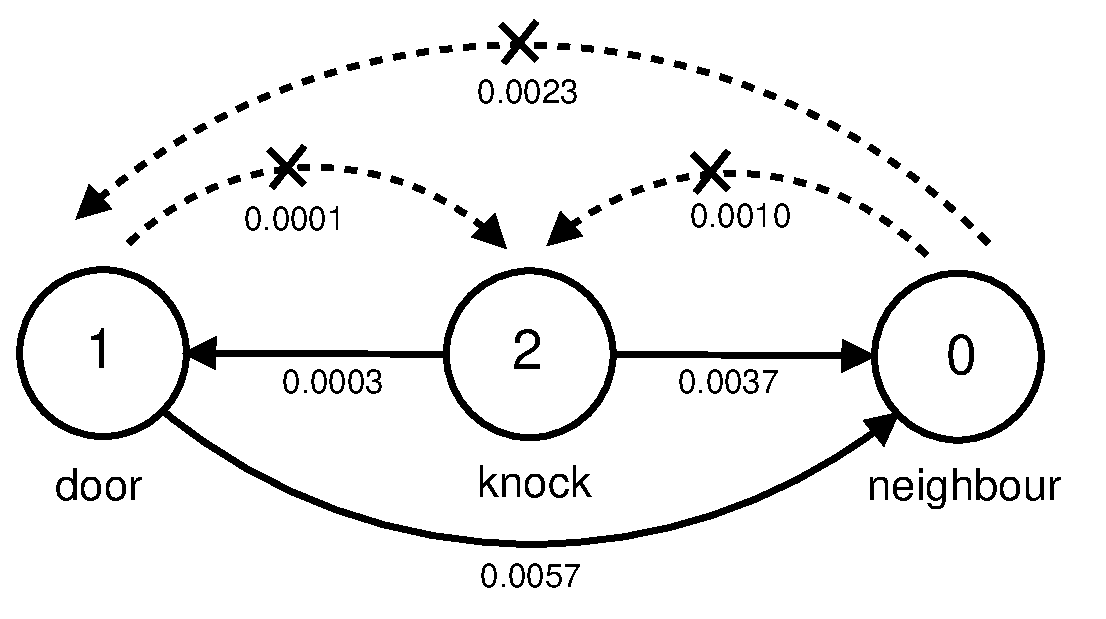
\epsfig{file=causeEvent.eps, width=0.6\columnwidth}
\caption{Weights in an event in a cause sentence}
\label{fig:causeEvent}
\end{figure}

\begin{figure}[th]
\centering
\epsfig{file=effectEvent.eps, width=0.4\columnwidth}
\caption{Weights of event in an effect sentence}
\label{fig:effectEvent}
\end{figure}

For the words in the extracted events, we perform the intra-sentence
enhancement to strengthen the causal signal of some important words.
Recall that in commonsense causal reasoning, we need to compute the
overall causal strength between the premise and an alternative. It
is known {\em a priori} whether the premise is a cause or an effect.
Therefore, when we extract event from an input sentence, which can
be either the premise or the alternative, we know whether the event
is to be a cause, which we call {\em cause event}, or an effect,
which we call {\em effect event}. We formulate events as
light-weight patterns to refine the causality score between two
sentences. In simple terms, it is a process of boosting weights of
cause words in cause events and effect words in effect events, by
assigning weights to words according to the the number of outgoing
and incoming edges. In \figref{fig:causeEvent}, which shows, as
an example, an event {\em knock-neighbor-door},
extracted from a cause sentence, there are
originally six edges among the three words, each carrying a \emph{CS}
score between the two adjacent words. For each pair of words in this
sub-graph, we remove the edge with a smaller score, and effectively
retain three edges (marked by solid lines) as a result. Then for
each word, we count the number of {\em outgoing} edges (since this
is a cause event), which acts as the weight for that word. In this
case, {\em knock} has weight 2, {\em neighbor} has weight 0, while
{\em door} has a weight of 1. Similarly weights can be computed by
counting the number of {\em incoming} edges for the effect event
{\em leave-house} in \figref{fig:effectEvent}.

We find this heuristic to be empirically useful, which
suggests that active cause/effect agents in sentences tend to be
more important for causality encoding. We leverage such contextual
information in sentences and build it into a light-weight causal
structure for event, such that the causal strength between any two
words will be boosted by their respective weights, which are computed
according to the above heuristic.

}%%%%%%%%%%%%%%% end of cut


%This may be even more helpful for longer and more complex sentences.
%= find proper examples =

%
%For example, we extract ``\emph{predict} \emph{high} \emph{temperature}''
%(*need to change*)as cause event, the light weighting pattern is shown as
%\figref{fig:causeEvent}.
%We extract `` \emph{cast} \emph{shadow} '' as effect event , the light weighting
%pattern is shown as \figref{}.
%
%which contains only two words, we compare two causal strength
%values modeled with $\alpha$-\textit{causality PMI}. If
%$\textit{PMI}_{\alpha\textit{-causality}}[\langle C(w1)\rightarrow
%E(w2)\rangle]$  $\textit{PMI}_{\alpha\textit{-causality}}[\langle
%C(w2)\rightarrow E(w1)\rangle]$ and specify the direction in such event.
%Like the example shown above, we compare the
%$\textit{PMI}_{\alpha\textit{-causality}}[\langle C(\textit{cut})\rightarrow
%E(\textit{half})\rangle]$ score of ``cut $\rightarrow$ half'' and
%"half$\rightarrow$cut" and then confirm that the direction comes from "cut" and
%goes to "half".
%
%(*How we formulate the light pattern within events?*)
%
%For events in cause sentences, we count the number of
%outgoing edges of one word as its weight in the event.
%And for events in effect sentences,
%we count the number of incoming edges of one word as its weight in the event.
%This is because words with more outgoing edges in cause sentence tend to be the initial reason of the event,
%which is the same for words with more incoming edges in effect sentence.
%By doing so, we strengthen the inner events and tune weights for event words.
%
%If there isn't a strong inner causality structure some events,
%boosting process based on causality score will usually lead to boosting verbs
%weights more of that event which is also reasonable, since verbs usually the
%most important of role of one sentence/event.
